\documentclass{article}

\def\npart{III}
\def\nyear{2018}
\def\nterm{Michaelmas}
\def\nlecturer{Dr. P. Varj\'{u}}
\def\ncourse{Topics in Ergodic Theory}
\def\draft{Ongoing course, rough}
\usepackage{imakeidx}
\ifx \nauthor\undefined
  \def\nauthor{Bhavik Mehta}
\else
\fi

\author{Based on lectures by \nlecturer \\\small Notes taken by \nauthor}
\date{\nterm\ \nyear}
\title{Part \npart\ -- \ncourse}

\usepackage[utf8]{inputenc}
\usepackage{amsmath}
\usepackage{amsthm}
\usepackage{amssymb}
\usepackage{enumerate}
\usepackage{mathtools}
\usepackage{graphicx}
\usepackage[dvipsnames]{xcolor}
\usepackage{tikz}
\usepackage{wrapfig}
\usepackage{centernot}
\usepackage{float}
\usepackage{braket}
\usepackage[hypcap=true]{caption}
\usepackage{enumitem}
\usepackage[colorlinks=true, linkcolor=mblue]{hyperref}
\usepackage[nameinlink,noabbrev]{cleveref}
\usepackage{nameref}
\usepackage[margin=1.5in]{geometry}

% Theorems
\theoremstyle{definition}
\newtheorem*{aim}{Aim}
\newtheorem*{axiom}{Axiom}
\newtheorem*{claim}{Claim}
\newtheorem*{cor}{Corollary}
\newtheorem*{conjecture}{Conjecture}
\newtheorem*{defi}{Definition}
\newtheorem*{eg}{Example}
\newtheorem*{ex}{Exercise}
\newtheorem*{fact}{Fact}
\newtheorem*{law}{Law}
\newtheorem*{lemma}{Lemma}
\newtheorem*{notation}{Notation}
\newtheorem*{prop}{Proposition}
\newtheorem*{question}{Question}
\newtheorem*{rrule}{Rule}
\newtheorem*{thm}{Theorem}
\newtheorem*{assumption}{Assumption}

\newtheorem*{remark}{Remark}
\newtheorem*{warning}{Warning}
\newtheorem*{exercise}{Exercise}

% \newcommand{\nthmautorefname}{Theorem}

\newtheorem{nthm}{Theorem}[section]
\newtheorem{nlemma}[nthm]{Lemma}
\newtheorem{nprop}[nthm]{Proposition}
\newtheorem{ncor}[nthm]{Corollary}
\newtheorem{ndef}[nthm]{Definition}

% Special sets
\newcommand{\C}{\mathbb{C}}
\newcommand{\N}{\mathbb{N}}
\newcommand{\Q}{\mathbb{Q}}
\newcommand{\R}{\mathbb{R}}
\newcommand{\Z}{\mathbb{Z}}

\newcommand{\abs}[1]{\left\lvert #1\right\rvert}
\newcommand{\norm}[1]{\left\lVert #1\right\rVert}
\renewcommand{\vec}[1]{\boldsymbol{\mathbf{#1}}}

\let\Im\relax
\let\Re\relax

\DeclareMathOperator{\Im}{Im}
\DeclareMathOperator{\Re}{Re}
\DeclareMathOperator{\id}{id}

\definecolor{mblue}{rgb}{0., 0.05, 0.6}

\makeindex[intoc]

% preamble

% and here we go!

\begin{document}
\maketitle

\tableofcontents

\clearpage
Ergodic theory is all about measure preserving systems.
\begin{defi}[Measure preserving system]\index{measure preserving!system}\hypertarget{def:mps}
  A \textbf{measure preserving system} $(X, \mathcal{B}, \mu, T)$ with $X$ a set, $\mathcal{B}$ a $\sigma$-algebra, $\mu$ a probability measure ($\mu(A) \geq 0$ $\forall A \in \mathcal{B}$ and $\mu(X) = 1$) and $T$ is a measure preserving transformation.
  \index{measure preserving!transformation}Recall a measure preserving transformation $T : X \to X$ is a measurable function such that $\mu(T^{-1}(A)) = \mu(A)$ $\forall A \in \mathcal{B}$.
\end{defi}
If $Y$ is a random element of $X$ with distribution $\mu$, then $T(Y)$ also has distribution $\mu$.

\begin{eg}
  \index{rotation map}For example, consider a circle rotation. We have $X = \mathbb{R}/\mathbb{Z}$, $\mathcal{B}$ is the Borel sets, $\mu$ the Lebesgue measure, and $T = R_\alpha$, with $x \mapsto x + \alpha$ and $\alpha \in \mathbb{R}/\mathbb{Z}$ is a parameter.

  \index{doubling map}\hypertarget{def:doubling}We also have the `times 2 map', with the same $X, \mathcal{B}, \mu$ and $T = T_2$, $x \mapsto 2 \cdot x$.
\end{eg}
\begin{proof}[Proof that \hyperlink{def:doubling}{$T_2$} is \hyperlink{def:mps}{measure preserving}]
  First check for intervals: Let $I = (a,b)$, then $\mu(I) = b-a$.
  Also, $\mu(T_2^{-1}I) = \mu\left((\frac{a}{2},\frac{b}{2}) \cup (\frac{a}{2} + \frac{1}{2}, \frac{b}{2} + \frac{1}{2})\right) = \frac{b}{2} - \frac{a}{2} + \frac{b}{2} - \frac{a}{2} = b - a$, as required.

  Now, let $U \subset \mathbb{R}/\mathbb{Z}$ be open. Then $U = I_1 \sqcup I_2 \sqcup \dotsb$ is a disjoint union of intervals:
  \begin{align*}
    \mu(T^{-1} U) &= \mu\left(\bigcup T^{-1} I_j\right) \\
                  &= \sum \mu(T^{-1} I_j) \\
                  &= \sum \mu(I_j) \\
                  &= \mu(U).
  \end{align*}

  Let $K \subset \mathbb{R}/\mathbb{Z}$ be a compact set.
  \begin{align*}
    \mu(T^{-1} K) = 1 - \mu((T^{-1} K)^c) = 1 - \mu(T^{-1} K^c) = 1 - \mu(K^c) = \mu(K).
  \end{align*}
  Now let $A \in \mathcal{B}$ be arbitrary. Let $\epsilon > 0$. $\exists U$ open and $\exists K$ compact such that $K \subset A \subset U$ and $\mu(U \setminus K) < \epsilon$.
  \begin{align*}
    \mu(K) = \mu(T^{-1} K) \leq \mu(T^{-1} A) \leq \mu(T^{-1} U) = \mu(U).
  \end{align*}
  We also have $\mu(K) \leq \mu(A) \leq \mu(U)$.
  Since $\mu(U) - \mu(K) < \epsilon$, $|\mu(A) - \mu(T^{-1}A)| < \epsilon$. $\epsilon$ was arbitrary, so $\mu(A) = \mu(T^{-1} A)$.
\end{proof}

The two examples generalise to the Haar measure on a topological group and to endomorphisms respectively.

In ergodic theory, we study the long term behaviour of orbits.
\begin{defi}[Orbit]\index{orbit}\hypertarget{def:orbit}
  The orbit of $x \in X$ is the sequence
  \begin{equation*}
    x, Tx, T^2 x, \dotsc
  \end{equation*}
\end{defi}
Some questions we might ask are:
\begin{itemize}
  \item Let $A \in \mathcal{B}$ and $x \in A$. Does the orbit of $x$ visit $A$ infinitely often? (Recurrence)
  \item What is the proportion of times $n$ such that $T^n x \in A$?
  \item What is $\mu(\set{x \in A | T^n x \in A})$ if $n$ is large? (Mixing property)
\end{itemize}

\begin{eg}
  Let $A = [0, \frac{1}{4}) \subset \mathbb{R}/\mathbb{Z}$. %]
  Then $\hyperlink{def:doubling}{T_2}^n x \in A \iff $ the $n+1$th and $n+2$th `binary digits' of $x$ are $0$.

  For some $x = 0.x_1 x_2 x_3 \dots_2$, $x \in A$ corresponds to $x_1, x_2$ both being 0 and the doubling map sends $x$ to $T_2x = x_2 x_3 \dots_2$, giving the required property above.

  For example, $x = \frac{1}{6} = 0.00101010\dots_2$ starts in $A$ but never comes back to $A$.
  Also, we have $\mu(\set{x \in A | T_2^n x}) = \frac{1}{16}$ if $n \geq 2$.
\end{eg}

\begin{eg}[Markov shift]\index{markov shift}\hypertarget{def:markovshift}
  Let $P_1, P_2, \dotsc, P_n$ be a probability vector. Let $A \in \mathbb{R}^{n \times n}_{\geq 0}$ be the `matrix of transition probabilities'.
  Assume
  \begin{equation*}
    A
    \begin{pmatrix}
      1 \\ 1 \\ \vdots \\ 1
    \end{pmatrix}
    =
    \begin{pmatrix}
      1 \\ 1 \\ \vdots \\ 1
    \end{pmatrix},
    \begin{pmatrix}
      P_1 & P_2 & \dots & P_n
    \end{pmatrix}
    A =
    \begin{pmatrix}
      P_1 & P_2 & \dots & P_n
    \end{pmatrix}
  \end{equation*}
  Take $X = \{1, \dotsc, n\}^\mathbb{Z}$, $\mathcal{B}$ the Borel $\sigma$-algebra generated by the product topology of the discrete topology on $\{1, \dotsc, n\}$, $T = \sigma$ the shift map: $(\sigma x)_m = x_{m+1}$.
  Finally, set the measure
  \begin{equation*}
    \mu(\set{x \in X | x_m = i_0, x_{m+1} = i_1, \dotsc, x_{m+n} = i_n}) = P_{i_0} a_{i_0 i_1} \dotsm a_{i_{n-1} i_n}.
  \end{equation*}
\end{eg}

\begin{thm}[Szemer\'{e}di]\index{Szemer\'{e}rdi's theorem}\hypertarget{thm:sze}
  Let $S \subset \mathbb{Z}$ of positive upper Banach density. That is,
  \begin{equation*}
    \bar{d}(S) \coloneqq \limsup_{N,M: M - N \to \infty} \frac{1}{M-N} \big| S \cap [N,M-1] \big|
  \end{equation*}
  and $\bar{d}(S) > 0$.
  Then $S$ contains arbitrarily long arithmetic progressions. That is, $\forall l, \exists a \in \mathbb{Z}, d \in \mathbb{Z}_{> 0}$,
  \begin{equation*}a, a+d, \dotsc, a+(l-1)d \in S.\end{equation*}
\end{thm}

\begin{thm}[Furstenberg, multiple recurrence]\index{Furstenberg's theorem}\hypertarget{thm:furs}
  Let $(X, \mathcal{B}, \mu, T)$ be a \hyperlink{def:mps}{measure preserving system}. Let $A \in \mathcal{B}$ such that $\mu(A) > 0$. Let $l \in \mathbb{Z}_{>0}$.
  Then
  \begin{equation*}
    \liminf_{N \to \infty} \frac{1}{N} \sum_{n=1}^N \mu(A \cap T^{-n} A \cap \dotsb \cap T^{-(l-1) n} A) > 0.
  \end{equation*}
\end{thm}

Let
\begin{itemize}
  \item $X = \{0, 1\}^\Z$
  \item $\mathcal{B}=$ Borel $\sigma$-algebra
  \item $\sigma=$ the \hyperlink{def:markovshift}{shift} map $\vec{x} \mapsto (x_{n+1})_n$
\end{itemize}
Let $ \vec{x}^S \in X$ be defined by
\begin{equation*}
  \vec{x}_n^S =
  \begin{cases}
    1 & n\in S\\
    0 & n \notin S.
  \end{cases}
\end{equation*}
Also let $A\in\beta$ be given by $A = \set{x\in X | x_0 = 1}$.
Observe then that
\begin{equation*}
  \vec{x}^S_n=1\iff n\in S\iff \sigma^n\vec{x}^S\in A\iff (\sigma^n\vec{x}^S)_0=1.
\end{equation*}

Let $\{M_m\}$ and $\{N_m\}$ be sequences s.t. $ M_n-N_m\to\infty $ and
\begin{equation*} \bar{d}(S) = \lim_{m\to\infty}\frac{1}{M_m-N_m}\left|S\cap[N_m,M_m-1]\right| \end{equation*}
Let
\begin{equation*}
  \mu_m = \frac{1}{M_m-N_m}\sum_{n=N_m}^{M_m-1}\delta_{\sigma^n\vec{x}^S}
\end{equation*}
where $\delta_x$ is a measure on $X$ defined as
\begin{equation*}
  \delta_x(B) =
  \begin{cases}
    1 & x\in B\\
    0 & x\notin B
  \end{cases}
\end{equation*}

Let $\mu$ be the weak limit of \emph{a} subsequence of $\mu_m$.
Note how the $\mu$ could be different dependent on subsequence choice.

\begin{defi}[Weak limit]
  Let $X$ be a compact metric space.
  Let $\mu_m$ be a sequence of Borel measures on $X$, and let $\mu$ be another Borel measure.
  Then $\mu_m$ converges weakly to $\mu$ if for any $f\in C(X)$, we have
  \begin{equation*}
    \lim _{n \to \infty} \int_X f \,d \mu_{n} = \int_X f \,d \mu.
  \end{equation*}
\end{defi}

\begin{thm}(Banach-Alaoglu, or Helly)
  Let $X$ be a compact metric space.
  Then $\mathcal{M}(X)$, the set of Borel probability measures on $X$, endowed with the topology of weak convergence, is compact and metrizable.
  That is, there is a weakly convergent subsequence in any sequence of Borel probability measures.
\end{thm}

\begin{lemma}
  $(X, \mathcal{B}, \mu, \sigma)$ as defined above is a \hyperlink{def:mps}{measure preserving system}.
\end{lemma}
\begin{proof}[Proof sketch]
  Let $B \in \mathcal{B}$. Then
  \begin{align*}
    \mu_m(B) &= \frac{1}{M_m - N_m} \left|\set{n \in [N_m, M_m -1] | \sigma^n \vec{x}^S \in \mathcal{B}} \right| \\
    \mu_m(\sigma^{-1} B) &= \frac{1}{M_m - N_m} \left|\set{n \in [N_m, M_m -1] | \sigma^n \vec{x}^S \in \sigma^{-1}\mathcal{B}} \right| \\
                         &= \frac{1}{M_m - N_m} \left|\set{n \in [N_m+1, M_m] | \sigma^n \vec{x}^S \in \mathcal{B}} \right|
  \end{align*}

  So the difference is such that
  \[ \left|\mu_m(B) - \mu_m(\sigma^{-1}B)\right| \leq \frac{1}{M_m-N_m}\to 0 \]
  It can be shown that we can pass to the limit on $ m $ and conclude that $ \mu(B) = \mu(\theta^{-1}B)$.
\end{proof}

\begin{remark}
  If $B$ is a cylinder set, i.e.\ $\exists L \in \mathbb{Z}_{>0}$ and $\tilde{B} \subseteq \{0,1\}^{2L+1}$ such that
  \begin{equation*}
    B = \set{x \in X | (x_{-L}, \dotsc, x_L) \in \tilde{B}},
  \end{equation*}
  then $B$ is both closed and open.
  Therefore $\chi_B$, the characteristic function of $B$ is continuous.
  Hence $\lim_{n \to \infty} \mu_m(B) = \mu(B)$, since $\mu_m(B) = \int \chi_B \, d \mu_m$ and $\mu(B) = \int \chi_B \, d \mu$.

  Approximating any Borel set by such cylinder sets would help complete the proof, but we in fact can get this result on spaces where $ \chi $ is not continuous on nice set of sets. So we leave full proof till a more general theorem.
\end{remark}

\begin{prop}
  Let $S \subseteq \mathbb{Z}$, let $\vec{x}^S, A, (X, \mathcal{B}, \mu, \sigma)$ as defined above.
  Let $l \in \mathbb{Z}_{> 0}$.
  Suppose that $\exists n \in \mathbb{Z}_{>0}$ such that
  \begin{equation*}
    \mu\left(A \cap \sigma^{-n}(A) \cap \dotsb \cap \sigma^{-n(l-1)}(A)\right) > 0.
  \end{equation*}
  Then $S$ contains an arithmetic progression of length $l$.
\end{prop}
\begin{proof}
  Without loss of generality, we can assume $\mu = \lim \mu_m$ - if not, pass to a subsequence.
  Let $B = A \cap \sigma^{-n} A \cap \dotsb \cap \sigma^{-n (l-1)} (A).$
  Observe that $B$ is a cylinder set.
  Then by the earlier remark, $\mu(B) = \lim \mu_m(B)$, hence $\exists m$ such that $\mu_m(B) > 0$.

  By definition of $\mu_m$, $\exists k \in [N_m, M_m - 1]$ such that $\sigma^k \vec{x}^S \in B$.
  Hence
  \begin{equation*}\sigma^k \vec{x}^S \in A, \sigma^k \vec{x}^S \in \sigma^{-n}(A), \dotsc, \sigma^k \vec{x}^S \in \sigma^{-n(l-1)}(A).\end{equation*}
  Thus, $k, k+n, \dotsc, k + n(l-1) \in S$.
\end{proof}
Returning to the overall proof, we note $ A $ is a cylinder set.
Then $ \mu_m(A)\to\mu(A) $, i.e.\
\begin{equation*} \mu(A) = \underbrace{\lim_{m\to\infty}\frac{1}{M_m-N_m}\left|\set{n\in[N_m,M_m-1]: n\in S}\right|}_{\bar{d}(S)} > 0 \end{equation*}
where the inequality comes from satisfying the conditions of Furstenberg.

\begin{lemma}
  Let $(X, \mathcal{B}, \mu, T)$ be a \hyperlink{def:mps}{measure preserving system}. Let $A \in \mathcal{B}$ with $\mu(A) > 0$. Then $\exists u \in \mathbb{Z}_{> 0}$ such that $\mu(A \cap T^{-n} A) > 0$.
\end{lemma}
\begin{proof}
  Suppose $\mu(A \cap T^{-n}A) = 0$ for all $n > 0$.
  Then $\mu(T^{-k}A \cap T^{-n} A) = \mu(A \cap T^{-(n-k)}A) = 0$ for all $n > k \geq 0$.

  Then the set $A, T^{-1} A, \dotsc$ are `almost pairwise disjoint'.
  Then
  \begin{align*}
    \mu(A \cup T^{-1} A \cup \dotsb \cup T^{-n} A) &= \mu(A) \\
                                                   &+ \mu(T^{-1} A) - \underbrace{\mu(T^{-1}A \cap A)}_{=0} \\
                                                   &+ \mu(T^{-2} A) - \underbrace{\mu(T^{-2} A \cap (A \cup T^{-1} A))}_{=0} \\
                                                   &+ \dotsb \\
                                                   &+ \mu(T^{-n} A) - \underbrace{\mu(T^{-n} A \cap (A \cup T^{-1} A \cup \dotsb \cup T^{-(n-1)} A))}_{=0} \\
                                                   &= (n+1) \mu(A),
  \end{align*}
  a contradiction if $n + 1 > \mu(A)^{-1}$.
\end{proof}
\begin{thm}[Poincar\'{e} recurrence]
  Let $(X, \mathcal{B}, \mu, T)$ be a \hyperlink{def:mps}{MPS}. Let $A \in \mathcal{B}$ with $\mu(A) > 0$. Then a.e.\ $x \in A$ returns to $A$ infinitely often.
  That is:
  \begin{equation*}
    \mu(A \setminus \bigcap_{N=1}^\infty \bigcup_{n=N}^\infty T^{-n} A) = 0.
  \end{equation*}
\end{thm}
\begin{remark}
  $x \in T^{-n} A \iff T^n x \in A$. $\bigcup_{n=N}^\infty T^{-n} A$ are the points that visit $A$ at least once after time $N$.
\end{remark}
\begin{proof}
  Let $A_0$ be the set of points in $A$ that never return to $A$. We first show $\mu(A_0) = 0$. Note that $\mu(A_0 \cap T^{-n} A_0) \leq \mu(A_0 \cap T^{-n} A) = \mu(\emptyset) = 0 \; \forall n > 0$.
  By the lemma, $\mu(A_0) = 0$. Note that if $x \in (A \setminus \cap_{N=1}^\infty \cup_{n=N}^\infty T^{-n} A)$, then there is a maximal $m \in \mathbb{Z}_{\geq 0}$ such that $T^m x \in A$.
  This means that
  \begin{equation*}
    A \setminus \bigcap \bigcup T^{-n} A \subset \bigcup_{m=0}^\infty T^{-m} A
  \end{equation*}
  where the right hand side has measure 0.
\end{proof}

This effectively answers one % which one
of the questions we asked earlier. % describe how

%What if the point does not start in $A$?
The main issue that can occur is that $X$ splits into parts, which are preserved under $T$:
\begin{center}
  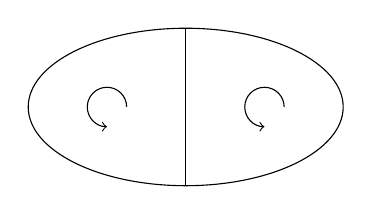
\begin{tikzpicture}
    \draw (0,0) circle[x radius=2cm, y radius=1cm];
    \draw (0,-1) -- (0,1);
    \draw [->] (-0.75,0) arc[radius=2.5mm, start angle= 0, end angle= 270];
    \draw [->] (1.25,0) arc[radius=2.5mm, start angle= 0, end angle= 270];
  \end{tikzpicture}
\end{center}

\begin{defi}[Ergodic]
  A \hyperlink{def:mps}{measure preserving system} is called \textbf{ergodic} if $A = T^{-1}A$ implies $\mu(A) = 0$ or $1$ for all $A \in \mathcal{B}$.
\end{defi}

If the MPS is not \hyperlink{def:ergodic}{ergodic}, and $A \in \mathcal{B}$ with $0 < \mu(A) < 1$ such that $T^{-1} A = A$, then we can restrict the MPS to $A$.
That is, we consider the MPS: $(A, \mathcal{B}_A, \mu_A, T|_A)$ where $\mathcal{B}_A = \set{B \in \mathcal{B} | B \subseteq A}$ and $\mu_A(B) = \frac{\mu(B)}{\mu(A)}$ for all $B \in \mathcal{B}_A$.
\begin{thm}
  The following are equivalent for an \hyperlink{def:mps}{measure preserving system} $(X, \mathcal{B}, \mu,T)$.
  \begin{enumerate}[label=(\arabic*)]
    \item $(X, \mathcal{B}, \mu, T)$ is \hyperlink{def:ergodic}{ergodic}.
    \item For all $A \in \mathcal{B}$ with $\mu(A) > 0$,
      \begin{equation*}
        \mu\left(\bigcap_{N=1}^\infty \bigcup_{n=N}^\infty T^{-n} A\right) = 1.
      \end{equation*}
    \item $\mu(A \triangle T^{-1} A) = 0$ implies $\mu(A) = 0$ or $1$ $\forall A \in \mathcal{B}$.
    \item For all bounded measurable functions $f: X \to \mathbb{R}$,
      $f = f \circ T$ a.e.\ implies $f$ is constant a.e.
    \item For all bounded measurable functions $f: X \to \mathbb{C}$,
      $f = f \circ T$ a.e.\ implies $f$ is constant a.e.
  \end{enumerate}
\end{thm}
\begin{proof}
  (1) $\Rightarrow$ (2). Let $A \in \mathcal{B}$ with $\mu(A) > 0$. Let $B = \bigcap \bigcup T^{-n}A$.
  By Poincar\'e recurrence, $\mu(B) \geq \mu(A) > 0$. So if we show that $B = T^{-1} B$, then $\mu(B) = 1$ follows by ergodicity.
  $x \in B$ iff $x$ visits $A$ infinitely often $\iff Tx$ visits $A$ infinitely often $\iff T_x \in B$.
  So we have proved $B = T^{-1} B$.

  (2) $\Rightarrow$ (3). Let $A \in \mathcal{B}$ such that $\mu(A \triangle T^{-1} A) = 0$. If $\mu(A) = 0$, there is nothing to prove. Suppose $\mu(A) > 0$.
  Let $B = \bigcap \bigcup T^{-n} A$. By (2), we know that $\mu(B) = 1$. We show $\mu(B \setminus A) = 0$, which completes the proof.
  Let $x \in B \setminus A$, then there is a first time $m$ such that $T^m x \in A$, and $m > 0$.
  Hence $x \in T^{-m} A \setminus T^{-(m-1)}A$. Thus
  \begin{equation*}
    B \setminus A \subseteq \bigcup_m T^{-m} A \setminus T^{-(m-1)} A,
  \end{equation*}
  and $\mu(T^{-m} A \setminus T^{-(m-1)} A) = \mu(T^{-1} A \setminus A) = 0$, so $\mu(B \setminus A) = 0$.

  (3) $\implies$ (4).
  Let $f : X \to \mathbb{R}$ be a bounded measurable function such that $f = f \circ T$ almost everywhere.
  For all $t \in \mathbb{R}$, let $A_t = \set{x \in X | f(x) \leq t}$.
  Then $\mu(A_t \triangle T^{-1} A_t) = 0$.
  By (3), we have $\mu(A_t) = 0$ or $1$ for all $t$.
  If $t$ is very small, then $\mu(A_t) = 0$. If $t$ is very large, $\mu(A_t) = 1$. $t \mapsto \mu(A_t)$ is monotone, hence $\exists c \in \mathbb{R}$ such that $\mu(A_t) = 0$ for all $t < c$ and $\mu(A_t) = 1 \; \forall t > c$.
  Then $f(x) = c$ a.e.

  (4) $\Leftrightarrow$ (5) is left as an exercise.
  (4) $\Rightarrow$ (1). Let $A \in \mathcal{B}$ with $A = T^{-1} A$. Then $\chi(A) = \chi(A) \circ T$ everywhere so $\chi(A)$ is constant a.e.
\end{proof}
\begin{eg}
  The circle rotation map $(\mathbb{R}/\mathbb{Z}, \mathcal{B}, \mu, R_\alpha)$ is ergodic iff $\alpha$ is irrational.
  Let $f: X \to \mathbb{R}$ be measurable. $f(x) = \sum_{n \in \mathbb{Z}} a_n \exp(2\pi i n x)$.
  \begin{align}
    f \circ R_\alpha(x) = f(x + \alpha) &= \sum_{n \in \mathbb{Z}} a_n \exp(2 \pi i n (x + \alpha)) \\
                                        &= \sum_{n \in \mathbb{Z}} a_n \exp(2\pi i n \alpha) \exp(2 \pi i n x)
  \end{align}
  So $f = f \circ R_\alpha \iff a_n = a_n = \exp(2 \pi i n \alpha) \; \forall n$. If $\alpha$ is irrational, then $\exp(2 \pi i n \alpha) \neq 1$ for all $n \neq 0$, then $a_n = 0$.
\end{eg}

\textbf{missing content here}
% loads of missing crap

\begin{thm}[Maximal ergodic theorem, Wiener]
  Let $(X, \mathcal{B}, \mu, T)$ be a \hyperlink{def:mps}{measure preserving system}.
  Let $f \in L^1$, $\alpha \in \mathbb{R}_{> 0}$. Let
  \begin{equation*}
    E_\alpha = \set{x \in X | \sup_{N > 0} \frac{1}{N} \sum_{n=0}^{N-1} f(T^n x) > \alpha}.
  \end{equation*}
  Then $\mu(E_\alpha) \leq \alpha^{-1} \|f\|_1$.
\end{thm}
\begin{prop}
  Let $(X, \mathcal{B},\mu,T)$ be a \hyperlink{def:mps}{measure preserving system}.
  Let $f \in L^1$. Let $f_0 = 0, f_1 = f, f_2 = f \circ T + f$,
  \begin{equation*}
    f_n = f \circ T^{n-1} + \dotsb + f \circ T + f,
  \end{equation*}
  and
  \begin{equation*}
    F_N = \max_{n = 0, \dotsc, N} f_n.
  \end{equation*}
  Then
  \begin{equation*}
    \int_{\set{x \in X | F_N(x) > 0}} f \, d \mu \geq 0 \; \forall N
  \end{equation*}
\end{prop}
\begin{proof}
  Suppose that $F_N(x) > 0$ for some $x$.
  Then $F_N(x) = f_n(x)$ for some $n \in \{1, \dotsc, N\}$.
  Then $F_N(x) = f_{n-1}(Tx) + f(x) \leq F_N(Tx) + f(x)$, hence
  $f(x) \geq F_N(x) - F_N(Tx)$.
  \begin{align*}
    \int_{\set{x \in X | F_N(x) > 0}} f(x)\,d\mu &\geq \int_{\set{x \in X | F_N(x) > 0}} (F_n(x) - F_N(Tx))\,d\mu \\
    \shortintertext{note if $F_n(x) \not> 0$, then $F_N(x) - F_N(Tx) \leq 0$, so}
                                                 & \geq \int_X F_N(x) - F_N(Tx)\,d\mu = 0
  \end{align*}
\end{proof}
\begin{proof}[Proof of maximal ergodic theorem]
  Define
  \begin{align*}
    E_{\alpha,M} &= \Set{x \in X | \max_{N = 1, \dotsc, M} \frac{1}{N} \sum_{n=0}^{N-1} f(T^n x) > \alpha} \\
                 &= \Set{x \in X | \max_{N = 1, \dotsc, M} \sum_{n=0}^{N-1} (f(T^n x) - \alpha) > 0}
  \end{align*}
  We apply the proposition for the function $f - \alpha$.
  Then
  \begin{equation*}
    \int_{E_{\alpha,M}} (f(x) - \alpha)\,d\mu \geq 0
  \end{equation*}
  Then
  \begin{equation*}
    \int_{E_{\alpha,M}} f(x)\,d\mu \geq \alpha \mu(E_{\alpha,M})
  \end{equation*}
  and $\int_{E_{\alpha,M}} \leq \|f\|_1$.
  Note that $E_\alpha = \bigcup_M E_{\alpha,M}$, and this is an increasing union.
\end{proof}

% let x,b,u,t be a mps. Let f in l1, then `E f* in L1, t invariant such that ...\to f*(x) pointwise ae
\begin{proof}[Proof of pointwise ergodic theorem]
  Fix $\epsilon > 0$.
  Then $\exists f_\epsilon \in L^2$, $e_{\epsilon,1} \in L^1$ such that $f = f_\epsilon + e_{\epsilon_1}$, and $\|e_{\epsilon,1}\| < \epsilon$.
  $\exists g_\epsilon \in L62$, $e_{\epsilon,2} \in L^1$ such that $f_\epsilon = P_T f_\epsilon + g_\epsilon \circ T - g_\epsilon + e_{\epsilon,2}$ and $\|e_{\epsilon,2}\|_1 < \epsilon$.

  Also, $\exists h_\epsilon \in L^\infty$, $e_{\epsilon, 3} \in L^1$ such that $g_\epsilon = h_\epsilon + e_{\epsilon,3}$ and $\|e_{\epsilon,3}\|_1 < \epsilon$.

  Thus, $f = P_T f_\epsilon + h_\epsilon \circ T - h_\epsilon + e_\epsilon$, where $e_\epsilon \in L^1$ with $\|e_\epsilon\|_1 < 4\epsilon$.

  \begin{equation*}
    \frac{1}{N} \sum_{n=0}^{N_1} f(T^nx) = P_T f_\epsilon(x) + \frac{1}{N} \left(h_\epsilon(T^N x) - h_\epsilon(x)\right) + \frac{1}{N} \sum_{n=0}^{N-1} e_\epsilon(T^nx).
  \end{equation*}
  Let
  \begin{equation*}E_{\epsilon,\alpha} = \set{x \in X | \limsup_{N \to \infty} \left|\frac{1}{N} \sum_{n=0}^\infty f(T^n x) - P_T f_\epsilon(x)\right| > \alpha}.\end{equation*}
  Applying the maximal ergodic theorem for the function $e_\epsilon$:
  \begin{equation*}
    \mu(E_{\epsilon,\alpha}) \leq \alpha^{-1} \|e_\epsilon\|_1 \leq \frac{4\epsilon}{\alpha}.
  \end{equation*}

  Let $F$ be the set of points $x$ such that $\frac{1}{N} \sum_{n=0}^{N-1} f(T^nx)$ does not converge at $x$.
  Then $F \subset \cup F_\alpha$ where
  \begin{equation*}
    F_\alpha = \set{x \in X | \limsup_{N_1, N_2 \to \infty} \left|\frac{1}{N_1} \sum_{n=0}^{N_1 - 1} f(T^n x) - \frac{1}{N_2} \sum_{n=0}^{N_2 - 1} f(T^n x)\right| > 2\alpha}.
  \end{equation*}
  Notice $F_\alpha \subset E_{\epsilon,\alpha}$ for all $\epsilon > 0$.
  $\mu(F_\alpha) \leq \mu(E_{\epsilon,\alpha}) \leq \frac{4\epsilon}{\alpha}$.
  Therefore $\mu(F_\alpha) = 0$.

  We can take a countable sequence of $\alpha$'s and conclude $\mu(F) = 0$>
  We proved that $\frac{1}{N} \sum_{n=0}^{N-1} f(T^n x) \to f^*(x)$ for some function $f^*$.

  By Fatou's lemma, $f^* \in L^1$.
  It remains to prove $f^*(x) = f^*(Tx)$ a.e.
  For a.e.\ $x$,
  \begin{align*}
    f^*(x) &= \lim_{N \to \infty} \frac{1}{N} \sum_{n=0}^{N-1} f(T^n x) \\
    f^*(Tx) &= \lim_{N \to \infty} \frac{1}{N} \sum_{n=0}^{N-1} f(T^{n+1} x) \\
     &= \lim_{N \to \infty} \frac{1}{N} \sum_{n=1}^{N} f(T^n x) \\
     &= \lim_{N \to \infty} \frac{1}{N-1} \sum_{n=1}^{N-1} f(T^n x) \\
     &= \lim_{N \to \infty} \frac{1}{N} \sum_{n=1}^{N-1} f(T^n x) \\
  \end{align*}
  Then $f^*(x) - f^*(Tx) = \lim \frac{1}{N} f(x) = 0$.
\end{proof}
\printindex
\end{document}
